\chapter{Обзор концепций, алгоритмов и программных средств по теме исследования}\label{ch:ch1}

\section{Визуальные языки программирования}\label{sec:ch1/sec1}

Для объяснения принципа работы программы, программисты часто используют
графические модели, вроде блок-схем и диаграмм UML. Ввиду удобства графических
обозначений, возникает интерес в использовании подобных нотаций для
написания компьютерных программ. Такую концепцию создания программного обеспечения
реализуют визуальные языки программирования.

\textbf{Визуальный язык программирования} -- язык программирования, 
который позволяет пользователю создавать программы, манипулируя элементами
программы графически, а не задавая их в виде текста \cite{maturityofvpl}.

Главное назначение визуальных языков программирования -- сделать 
программирование более доступным людей без опыта с ним,
улучшить пользовательских опыт программиста на трёх уровнях \cite{agentsheetsmovingbeyondsyntax}:

\begin{itemize}
    \item \textbf{На уровне синтаксиса} -- элементы визуальных языков вместо текста 
    представлены строго в виде пиктограмм, блоков, диаграмм, что исключает возможность
    наличия в программе синтаксических ошибок.
    \item \textbf{На уровне семантики} -- графическое представление объектов
    языка позволяет наглядно показать назначение программных примитивов, тем
    самым сокращает время обучения языку.
    \item \textbf{На прикладном уровне} -- многие визуальные языки позволяют
    перевести программу в определенное состояние с целью изучения, как поведет
    себя программа в данном состоянии.
\end{itemize}

\section{Типы визуальных языков программирования}\label{sec:ch1/sec2}

\subsection{Блочные языки}\label{sech:ch1/sec2/sub1}

Блочные языки позволяют составлять программы из блоков-инструкций.
Управляющие конструкции блочных языков в целом копируют классические языки,
но графические подсказки помогают понять, как комбинировать базовые элементы,
такие как переменные, инструкции управления потоком выполнения. В блоках
используются текстовые обозначения для задания имен и значений переменных.

В сравнении с другими графическими языками, программы на блочных языках
близки к исходному коду на императивных языках, но использование
визуальных блоков позволяет избежать ошибок за счет ограничений языка.

На рисунке~\ref{fig:blockly} приведен пример программы, три раза выводящей
на экран сообщение <<Hello World!>>, на блочном языке Blocky \cite{blocklysite}.
\begin{figure}[ht]
	\centering
	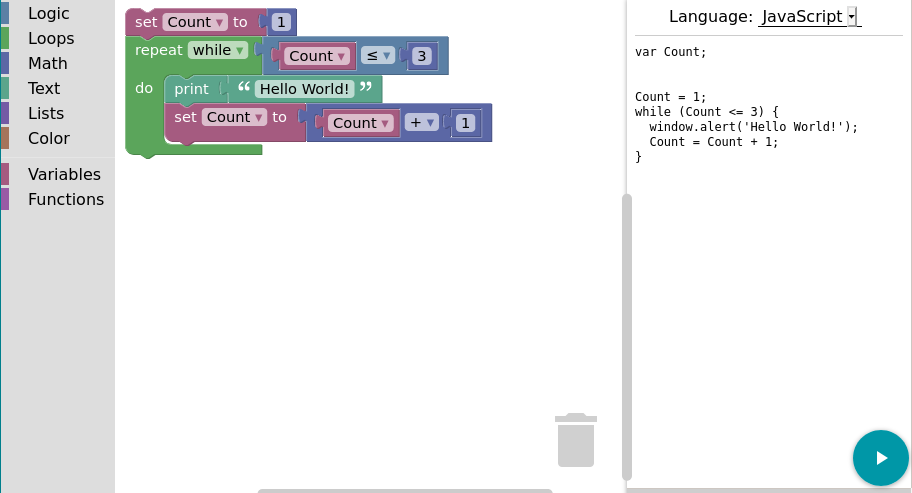
\includegraphics [scale=0.65] {blockly}
	\caption{Пример программы на блочном языке}
	\label{fig:blockly}
\end{figure}

\subsection{Языки, основанные на блок-схемах}\label{sech:ch1/sec2/sub2}

Существуют визуальные языки, использующие представление, близкое к
блок-схемам, для описания главного потока управления программы. Программы
на таких языках представлены набором блоков, соединенных между собой линиями, 
задающими последовательность исполнения инструкций.

Простая визуальная грамматика и упор на исполнение программ делают такие
языки легкими в освоении, однако программы на таких языках быстро
разрастаются и становятся трудночитаемыми.

На рисунке~\ref{fig:flowgorithm} приведен пример программы 
на языке Flowgorithm \cite{flowgorithm}, основанном на блок-схемах.
\begin{figure}[ht]
	\centering
	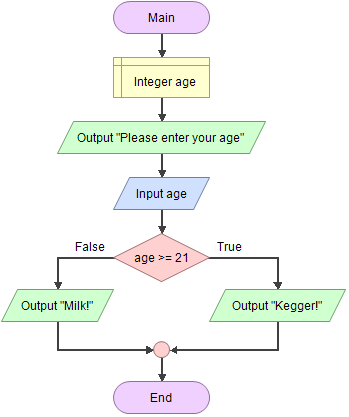
\includegraphics [scale=0.65] {flowgorithm}
	\caption{Пример программы на языке, основанном на блок-схемах}
	\label{fig:flowgorithm}
\end{figure}

\subsection{Языки программирования потоков данных}\label{sech:ch1/sec2/sub3}

Наиболее часто в профессиональных программных комплексах используются
визуальные языки программирования потоков данных. Как правило, такие
языки ориентированы на специалистов, не использующих текстовые языки
программирования в своей повседневной работе.

В программировании потока данных блок представляют функции, связанные
с собой потоком данных, от входа к выходу. Создавая связи между
точкой выхода одного блока и точкой входа другого блока, программист
задает поток выполнения программы через поток данных.

Множество процессов реальной жизни может быть промоделировано с помощью
потоков данных, поэтому визуальные языки подобного рода часто 
используются как встраиваемые языки предметной области в сложных
конфигурируемых программных продуктах: системах потоковой обработки
информации, игровых движках, пакетах компьютерной графики.

На рисунке~\ref{fig:blueprint} приведен пример программы 
на языке программирования потоков данных Blueprint \cite{blueprint}, 
используемого для создания пользовательских сценариев в игровом движке
Unreal Engine 4.
\begin{figure}[ht]
	\centering
	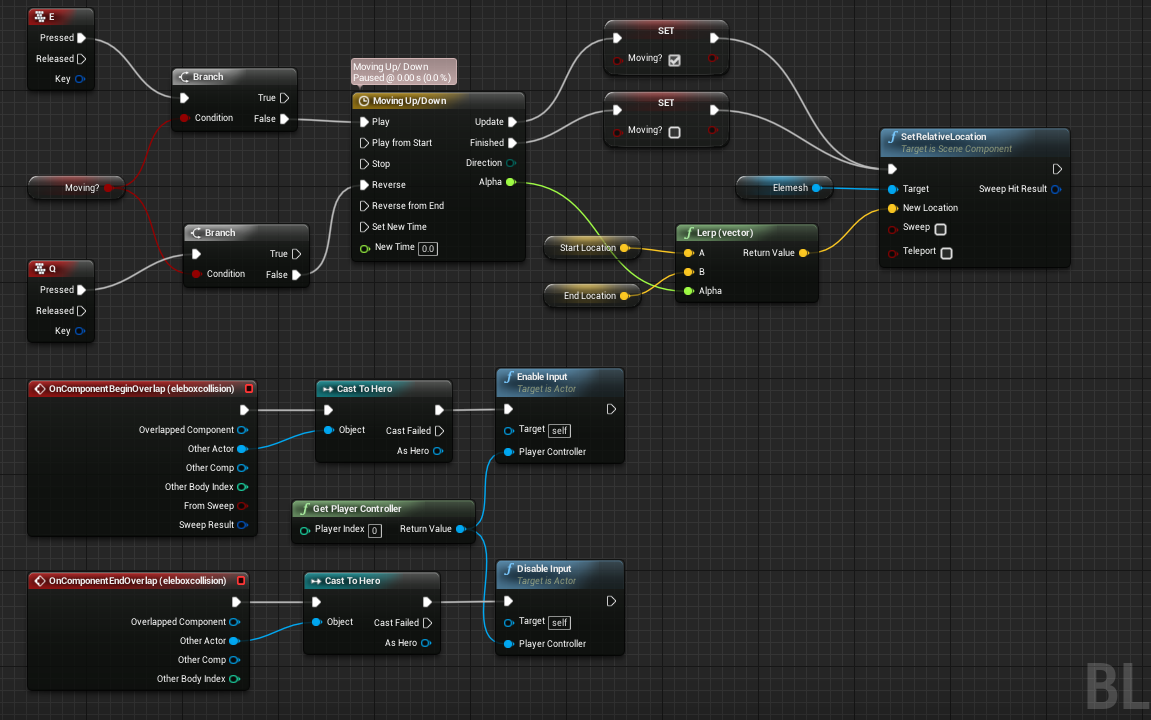
\includegraphics [scale=0.45] {blueprint}
	\caption{Пример программы на языке программирования потоков данных}
	\label{fig:blueprint}
\end{figure}

\section{Функциональное программирование}\label{sec:ch1/sec3}

В информатике функциональное программирование --- это парадигма программирования, в которой программы создаются путем применения и композиции функций. Это декларативная парадигма программирования, в которой определения функций представляют собой деревья выражений, которые отображают значения в другие значения, а не последовательность императивных операторов, обновляющих текущее состояние программы.

В функциональном программировании функции рассматриваются как <<объекты первого класса>> (англ. --- first-class objects), что означает, что они могут быть привязаны к именам (включая локальные идентификаторы), передаваться в качестве параметров и возвращаться из других функций, как и любой другой тип данных. Это позволяет писать программы в декларативном и компонуемом стиле, в котором небольшие функции объединяются по модульному принципу.

Функциональное программирование иногда рассматривается как синоним чисто функционального программирования, подмножества функционального программирования, которое рассматривает все функции как детерминированные математические функции или чистые функции. Когда чистая функция вызывается с некоторыми заданными аргументами, она всегда будет возвращать один и тот же результат, и на нее не могут повлиять никакие изменяемые состояния или другие побочные эффекты. Это контрастирует с нечистыми процедурами, обычными для императивного программирования, которые могут иметь побочные эффекты (например, изменение состояния программы или получение данных от пользователя). Сторонники чисто функционального программирования утверждают, что за счет ограничения побочных эффектов программы могут иметь меньше ошибок, их легче отлаживать и тестировать, и они больше подходят для формальной проверки. 

\subsection{Функции высшего порядка}\label{sec:ch1/sec3/subsec1}

Функции высшего порядка - это функции, которые могут либо принимать другие функции в качестве аргументов, либо возвращать их в качестве результатов.

Функции высшего порядка тесно связаны с функциями первого класса в том смысле, что и функции высшего порядка, и функции первого класса допускают функции как аргументы и результаты других функций. Различие между ними тонкое: «высший порядок» описывает математическую концепцию функций, которые работают с другими функциями, в то время как «первоклассный» --- это термин в информатике для сущностей языка программирования, которые не имеют ограничений на их использование (таким образом, <<первоклассные>> функции могут появляться в любом месте программы, в отличие от других первоклассных сущностей, таких как числа, в том числе как аргументы для других функций и как их возвращаемые значения).

Функции высшего порядка допускают частичное приложение или каррирование, метод, который применяет функцию к ее аргументам по одному, причем каждое приложение возвращает новую функцию, которая принимает следующий аргумент. Это позволяет программисту кратко выразить, например, функцию следования как оператор сложения, частично примененный к натуральному числу один. 

\subsection{Чистые функции}\label{sec:ch1/sec3/subsec2}

Чистые функции (или выражения) не имеют побочных эффектов (памяти или ввода-вывода). Это означает, что чистые функции имеют несколько полезных свойств, многие из которых можно использовать для оптимизации кода: 

\begin{itemize}
    \item Если результат чистого выражения не используется, его можно удалить, не затрагивая другие выражения. 
    \item Если чистая функция вызывается с аргументами, которые не вызывают побочных эффектов, результат постоянен по отношению к этому списку аргументов (иногда называемый ссылочной прозрачностью или идемпотентностью), то есть повторный вызов чистой функции с теми же аргументами возвращает тот же результат. (Это может включить оптимизацию кеширования, например мемоизацию.) 
    \item Если между двумя чистыми выражениями нет зависимости данных, их порядок может быть изменен на противоположный или они могут выполняться параллельно, и они не могут мешать друг другу (другими словами, вычисление любого чистого выражения является потоко-безопасным). 
    \item Если весь язык не допускает побочных эффектов, можно использовать любую стратегию оценки; это дает компилятору свободу переупорядочивать или комбинировать вычисление выражений в программе. 
\end{itemize}

Хотя большинство компиляторов для императивных языков программирования обнаруживают чистые функции и выполняют исключение общих подвыражений для чистых вызовов функций, они не всегда могут делать это для предварительно скомпилированных библиотек, которые обычно не раскрывают эту информацию, тем самым предотвращая оптимизацию, включающую эти внешние функции. Некоторые компиляторы, такие как $gcc$, добавляют дополнительные ключевые слова для программиста, чтобы явно пометить внешние функции как чистые, чтобы включить такую оптимизацию. $Fortran 95$ также позволяет обозначать функции как «чистые». 

\subsection{Ссылочная прозрачность}\label{sec:ch1/sec3/subsec3}

Функциональные программы не имеют операторов присваивания, то есть значение переменной в функциональной программе никогда не изменяется после определения. Это исключает возможность возникновения побочных эффектов, поскольку любую переменную можно заменить ее фактическим значением в любой момент выполнения. Итак, функциональные программы ссылочно прозрачны. 

\subsection{Функциональные структуры данных}\label{sec:ch1/sec3/subsec4}

Чисто функциональные структуры данных часто представляются иначе, чем их императивные аналоги. Например, массив с постоянным временем доступа и обновления является базовым компонентом большинства императивных языков, а многие императивные структуры данных, такие как хеш-таблица и двоичная куча, основаны на массивах. Массивы могут быть заменены картами или списками произвольного доступа, которые допускают чисто функциональную реализацию, но имеют логарифмическое время доступа и обновления. Чисто функциональные структуры данных обладают постоянством, свойством сохранять неизменными предыдущие версии структуры данных.

\section{Elm-архитектура}\label{sec:ch1/sec4}

Elm-архитектура --- это шаблон для создания интерактивных программ, таких как веб-приложения и игры. 

Структурно Elm-архитектуру можно представить следующим образом: 

\begin{figure}[ht]
	\centering
	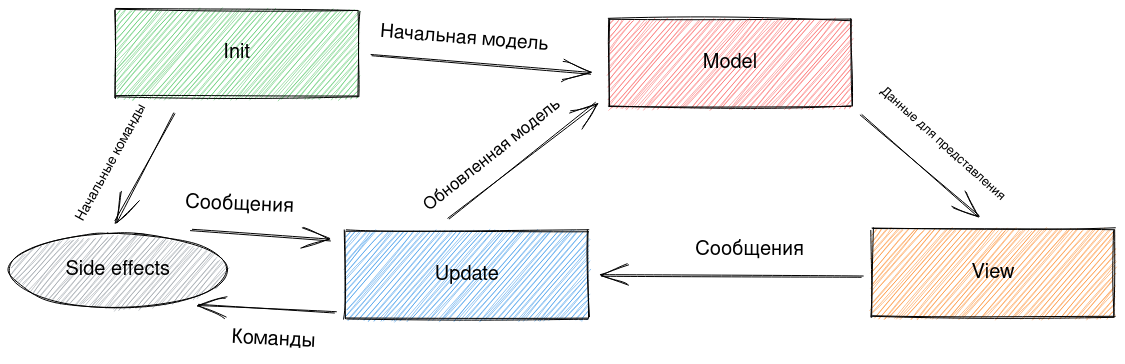
\includegraphics [scale=0.45] {elmarch}
	\caption{Структурная схема Elm-архитектуры}
	\label{fig:elmarch}
\end{figure}

\begin{itemize}
    \item Сообщение --- тип-сумма, значениями которого обмениваются блоки программы.
    \item Команда --- сообщение, посылаемое блоку побочных эффектов (HTTP-запросы, случайные числа и т.д.).
    \item Model --- описание данных программы. Просто тип данных - примитивный или составной.
    \item View --- отображение данных, представляется как чистая функция. Принимает модель из источника, строит и отображает документ. Если с документом совершено какое-либо пользовательское действие (нажали на кнопку, набрали текст в поле ввода), порождает сообщение, которое отправится в Update.
    \item Update --- функция, преобразующая модель и порождающая команды для блока побочных эффектов по полученным сообщениям.
    \item Init --- <<конструктор>> модели --- создает первую версию модели и порождает первые команды блоку побочных эффектов.
\end{itemize}

Цикл жизни программы, построенной с использованием Elm-архитектуры:

\begin{enumerate}
    \item Функция Init порождает модель, которая отображается функцией представления View.
    \item При наступлении пользовательского события View посылает сообщение на обновление модели Update.
    \item Update создает новую модель в соответствии с сообщением и посылает на отображение View.
\end{enumerate}

Работа с побочными эффектами осуществляется следующим образом:

\begin{enumerate}
    \item При наступлении пользовательского события View посылает сообщение на порождение команды Update.
    \item Update порождает команду для блока побочных эффектов.
    \item Происходит обработка побочного эффекта, результат посылается в Update сообщением.
    \item Update строит новую модель и передает View.
\end{enumerate}

\FloatBarrier

\section{Компиляторы}\label{sec:ch1/sec5}

В информатике компилятор --- это компьютерная программа, которая переводит компьютерный код, написанный на одном языке программирования (исходный язык), на другой язык (целевой язык). Название <<компилятор>> в основном используется для программ, которые переводят исходный код с языка программирования высокого уровня на язык более низкого уровня (например, язык ассемблера, объектный код или машинный код) для создания исполняемой программы. 

Есть много разных типов компиляторов, которые производят вывод в различных полезных формах. Компилятор, который может работать на компьютере, процессор или операционная система которого отличается от того, на котором будет выполняться создаваемый им код, называется кросс-компилятором. Компилятор начальной загрузки написан на языке, который он собирается компилировать. Программа, которая переводит с языка низкого уровня на язык более высокого уровня, является декомпилятором. Программа, которая осуществляет перевод между языками высокого уровня, обычно называется компилятором исходного кода или транскомпилятором. Переписчик языка - это обычно программа, которая переводит форму выражений без изменения языка. Термин «компилятор-компилятор» относится к инструментам, используемым для создания синтаксических анализаторов, выполняющих синтаксический анализ.

Компилятор может выполнять многие или все следующие операции: предварительную обработку, лексический анализ, синтаксический анализ, семантический анализ (синтаксически-управляемый перевод), преобразование входных программ в промежуточное представление, оптимизацию кода и генерацию кода. Компиляторы реализуют эти операции поэтапно, что способствует эффективному проектированию и правильному преобразованию исходного ввода в целевой вывод. Ошибки программы, вызванные неправильным поведением компилятора, очень сложно отследить и обойти; поэтому разработчики компилятора прилагают значительные усилия для обеспечения его корректности.

Компилятор осуществляет формальное преобразование исходной программы высокого уровня в целевую программу низкого уровня. Дизайн компилятора может определять сквозное решение или заниматься определенным подмножеством, которое взаимодействует с другими инструментами компиляции, например. препроцессоры, ассемблеры, линкеры. Требования к дизайну включают строго определенные интерфейсы как внутри между компонентами компилятора, так и снаружи между вспомогательными наборами инструментов.

Вначале подход к проектированию компилятора напрямую зависел от сложности обрабатываемого компьютерного языка, опыта человека (лиц), разрабатывающего его, и имеющихся ресурсов. Ограниченность ресурсов привела к необходимости повторять исходный код более одного раза.

Компилятор для относительно простого языка, написанный одним человеком, может быть единым монолитным программным обеспечением. Однако по мере того, как исходный язык становится все сложнее, дизайн может быть разделен на несколько взаимозависимых фаз. Отдельные этапы обеспечивают улучшения дизайна, которые фокусируют разработку на функциях в процессе компиляции. 

\subsection{Структура трёхпроходного компилятора}\label{sec:ch1/sec5/subsec1}

Независимо от точного количества этапов в конструкции компилятора, этапы можно отнести к одному из трех этапов. Этапы включают в себя фронт-энд (англ. --- fronte nd), миддл-энд (англ. --- middle end) и бэк-энд (англ. --- back end).

\begin{itemize}
    \item Фронт-энд сканирует ввод и проверяет синтаксис и семантику в соответствии с определенным исходным языком. Для языков со статической типизацией он выполняет проверку типа путем сбора информации о типе. Если входная программа синтаксически неверна или имеет ошибку типа, она генерирует сообщения об ошибках и / или предупреждения, обычно идентифицируя место в исходном коде, где была обнаружена проблема; в некоторых случаях фактическая ошибка может быть (намного) раньше в программе. Аспекты внешнего интерфейса включают лексический анализ, синтаксический анализ и семантический анализ. Внешний интерфейс преобразует входную программу в промежуточное представление (IR) для дальнейшей обработки средним концом. Этот IR обычно является представлением программы более низкого уровня по отношению к исходному коду. 
    \item Миддл-энд выполняет оптимизацию IR, которая не зависит от целевой архитектуры ЦП. Эта независимость исходного кода / машинного кода предназначена для обеспечения возможности совместной оптимизации между версиями компилятора, поддерживающими разные языки и целевые процессоры. Примерами оптимизации среднего уровня являются удаление бесполезного (устранение мертвого кода) или недоступного кода (анализ достижимости), обнаружение и распространение постоянных значений (распространение констант), перемещение вычислений в менее часто выполняемое место (например, вне цикла). , или специализация вычислений в зависимости от контекста. В конечном итоге создание «оптимизированного» IR, используемого бэк-эндом.
    \item Бэк-энд получает оптимизированное внутреннее представление от миддл-энда. Он может выполнять больше анализа, преобразований и оптимизаций, специфичных для целевой архитектуры ЦП. Бэк-энд генерирует зависимый от целевой платформы ассемблерный код, выполняя выделение регистров в процессе. Бэк-энд выполняет планирование инструкций, которое переупорядочивает инструкции, чтобы держать блоки параллельного выполнения занятыми, заполняя интервалы задержки. Хотя большинство задач оптимизации являются NP-трудными, эвристические методы их решения хорошо разработаны и в настоящее время реализованы в компиляторах производственного качества. Обычно выходные данные бэк-энда представляют собой машинный код, специализированный для конкретного процессора и операционной системы.  
\end{itemize}

\subsection{Фронт-энд компилятора}\label{sec:ch1/sec5/subsec2}

Фронт-энд анализирует исходный код для построения внутреннего представления программы, называемого промежуточным представлением (IR). Он также управляет таблицей символов, структурой данных, сопоставляющей каждый символ в исходном коде со связанной информацией, такой как местоположение, тип и область действия.

Хотя фронт-энд может быть отдельной монолитной функцией или программой, как в парсере без сканирования, он традиционно реализовывался и анализировался как несколько этапов, которые могут выполняться последовательно или одновременно. Этому методу отдают предпочтение из-за его модульности и разделения задач. Чаще всего сегодня интерфейс разбивается на три этапа: лексический анализ (также известный как лексирование или сканирование), синтаксический анализ (также известный как сканирование или синтаксический анализ) и семантический анализ. Лексирование и синтаксический анализ включают синтаксический анализ (синтаксис слов и синтаксис фраз соответственно), и в простых случаях эти модули (лексический анализатор и синтаксический анализатор) могут быть автоматически сгенерированы из грамматики языка, хотя в более сложных случаях они требуют ручной модификации. . Лексическая грамматика и грамматика фраз обычно являются контекстно-независимыми грамматиками, что значительно упрощает анализ, а контекстная чувствительность обрабатывается на этапе семантического анализа. Этап семантического анализа, как правило, более сложен и написан вручную, но может быть частично или полностью автоматизирован с использованием грамматик атрибутов. Сами эти этапы могут быть далее разбиты: лексирование как сканирование и оценка и анализ как построение конкретного синтаксического дерева (CST, дерево синтаксического анализа) с последующим преобразованием его в абстрактное синтаксическое дерево (AST, синтаксическое дерево). В некоторых случаях используются дополнительные фазы, в частности реконструкция линии и предварительная обработка, но это случается редко. 

\subsection{Миддл-энд компилятора}\label{sec:ch1/sec5/subsec3}

Миддл-энд, также известный как оптимизатор, выполняет оптимизацию промежуточного представления, чтобы улучшить производительность и качество производимого машинного кода. Миддл-энд содержит те оптимизации, которые не зависят от целевой архитектуры ЦП. 

Анализ компилятора является предпосылкой для любой оптимизации компилятора, и они тесно взаимодействуют друг с другом. Например, анализ зависимостей имеет решающее значение для преобразования цикла.

Объем анализа и оптимизации компилятора сильно различается; их объем может варьироваться от работы в пределах базового блока до целых процедур или даже всей программы. Существует компромисс между степенью детализации оптимизации и стоимостью компиляции. Например, оптимизация с помощью глазка выполняется быстро во время компиляции, но влияет только на небольшой локальный фрагмент кода и может выполняться независимо от контекста, в котором появляется фрагмент кода. Напротив, межпроцедурная оптимизация требует большего времени компиляции и объема памяти, но обеспечивает оптимизацию, которая возможна только при одновременном рассмотрении поведения нескольких функций. 

\subsection{Бэк-энд компилятора}\label{sec:ch1/sec5/subsec4}

Бэк-энд отвечает за оптимизацию кода под архитектуру ЦП и генерацию кода. 

Основные этапы бэкенда включают следующее: 

\begin{itemize}
    \item Машинно-зависимые оптимизации: оптимизации, которые зависят от деталей архитектуры ЦП, на которую нацелен компилятор. Ярким примером является оптимизация типа <<Дверной глазок>> (англ. -- peephole optimization), которая переписывает короткие последовательности инструкций ассемблера в более эффективные инструкции. 
    \item Генерация кода: преобразованный промежуточный язык переводится на выходной язык, обычно на собственный машинный язык системы. Это включает в себя решения о ресурсах и хранении, такие как решение, какие переменные вписываются в регистры и память, а также выбор и планирование соответствующих машинных инструкций вместе с соответствующими режимами адресации. Также может потребоваться сгенерировать данные отладки для облегчения отладки. 
\end{itemize}

\section{Рекурсия}\label{sec:ch1/sec6}

В информатике рекурсия --- это метод решения проблемы, решение которой зависит от решения более мелких экземпляров одной и той же проблемы. Такие проблемы, как правило, можно решить итерацией, но для этого необходимо идентифицировать и индексировать более мелкие экземпляры во время программирования. Рекурсия решает такие рекурсивные проблемы с помощью функций, которые вызывают себя из собственного кода. Этот подход может применяться ко многим типам задач, и рекурсия является одной из центральных идей информатики. 

Распространенная тактика компьютерного программирования --- разделить проблему на подзадачи того же типа, что и исходная, решить эти подзадачи и объединить результаты. Это часто называют методом <<разделяй и властвуй>>; в сочетании с таблицей поиска, в которой хранятся результаты ранее решенных подзадач (чтобы избежать их повторного решения и увеличения времени вычислений), это можно назвать динамическим программированием или мемоизацией.

Определение рекурсивной функции имеет один или несколько базовых случаев, то есть входные данные, для которых функция производит тривиальный результат (без повторения), и один или несколько рекурсивных случаев, то есть входные данные, для которых программа повторяется (вызывает саму себя). Например, функция вычисления факториала может быть определена рекурсивно. Ни одно уравнение само по себе не составляет полного определения; первый - базовый случай, второй - рекурсивный. Поскольку базовый случай разрывает цепочку рекурсии, его иногда также называют <<завершающим случаем>>.

Работа с рекурсивными случаями можно рассматривать как разбиение сложных входных данных на более простые. В правильно спроектированной рекурсивной функции при каждом рекурсивном вызове проблема ввода должна быть упрощена таким образом, чтобы в конечном итоге был достигнут базовый случай. (Функции, которые не предназначены для завершения при нормальных обстоятельствах --- например, некоторые системные и серверные процессы --- являются исключением.) Игнорирование написания базового варианта или его неправильное тестирование может вызвать бесконечный цикл. 

\section{Методы оптимизации рекурсии}\label{sec:ch1/sec7}

Итерация (цикл) в функциональных языках обычно выполняется с помощью рекурсии. Рекурсивные функции вызывают сами себя, позволяя операции повторяться до тех пор, пока она не достигнет базового случая. В общем, рекурсия требует поддержки стека, который занимает пространство линейно в зависимости от глубины рекурсии. Это может сделать рекурсию слишком дорогой в использовании вместо императивных циклов. Однако специальная форма рекурсии, известная как хвостовая рекурсия, может быть распознана и оптимизирована компилятором в тот же код, который используется для реализации итерации в императивных языках. Оптимизация хвостовой рекурсии может быть реализована путем преобразования программы в стиль передачи продолжения во время компиляции, среди других подходов.

Стандарт языка Scheme требует, чтобы реализации поддерживали правильную хвостовую рекурсию, то есть они должны допускать неограниченное количество активных хвостовых вызовов. Правильная хвостовая рекурсия - это не просто оптимизация; это языковая функция, которая гарантирует пользователям, что они могут использовать рекурсию для выражения цикла, и это будет безопасно для места. Более того, вопреки своему названию, он учитывает все хвостовые вызовы, а не только хвостовую рекурсию. Хотя правильная хвостовая рекурсия обычно реализуется путем превращения кода в императивные циклы, реализации могут реализовывать это другими способами. Например, диалект Chicken Scheme намеренно поддерживает стек и позволяет стеку переполняться. Однако, когда это происходит, его сборщик мусора потребует обратно пространство, позволяя неограниченное количество активных хвостовых вызовов, даже если он не превращает хвостовую рекурсию в цикл.

Общие шаблоны рекурсии могут быть абстрагированы с помощью функций высшего порядка, наиболее очевидными примерами которых являются катаморфизмы и анаморфизмы (или <<свёртки>> и <<развёртки>>). Такие рекурсивные схемы играют роль, аналогичную встроенным управляющим структурам, таким как циклы в императивных языках.

Большинство языков функционального программирования общего назначения допускают неограниченную рекурсию и являются полными по Тьюрингу, что делает проблему остановки неразрешимой, может вызвать несостоятельность эквациональных рассуждений и, как правило, требует внесения несогласованности в логику, выраженную системой типов языка. Некоторые языки специального назначения, такие как Coq, допускают только хорошо обоснованную рекурсию и строго нормализуют. Как следствие, эти языки не могут быть полными по Тьюрингу, и выражение в них определенных функций невозможно, но они по-прежнему могут выражать широкий класс интересных вычислений, избегая проблем, связанных с неограниченной рекурсией. Функциональное программирование, ограниченное хорошо обоснованной рекурсией с некоторыми другими ограничениями, называется полным функциональным программированием. 

%\section{Обзор связанных программных средств}\label{sec:ch1/sec8}

\section{Постановка задач на исследование}\label{sec:ch1/sec9}

В результате анализа технологий, методов, алгоритмов, была поставлена следующая цель:

\begin{itemize}
    \item Проектирование и разработка интегрированной среды программирования на визуальном функциональном языке с возможностью оптимизации рекурсии.
\end{itemize}

Были выделены следующие задачи:

\begin{enumerate}
    \item Анализ методов построения визуальных языков программирования и их компиляторов.
    \item Анализ технологий и алгоритмов оптимизации рекурсии на этапе компиляции программ <<миддл-энд>>.
    \item Проектирование визуального языка функционального программирования.
    \item Проектирование и разработка интегрированной среды визуального программирования на ранее спроектированном языке.
    \item Проектировани и разработка оптимизирующего компилятора программ на ранее спроектированном языке с транслятором в код на языке JavaScript в качестве целевой платформы.
\end{enumerate}

\nocite{*}

\FloatBarrier